\documentclass[a4paper,10 pt]{article} 

\usepackage{amsmath}
\usepackage{amssymb}
\usepackage[top = 2.5cm, bottom = 2.5cm, left = 2.5cm, right = 2.5cm]{geometry} 
\usepackage[T1]{fontenc}
\usepackage[utf8]{inputenc}
\usepackage{multirow} 
\usepackage{booktabs} 
\usepackage{graphicx} 
\usepackage[shortlabels]{enumitem}
\usepackage{setspace}
\setlength{\parindent}{0in}
\usepackage{float}
\usepackage{fancyhdr}
\usepackage{hyperref}
\usepackage{lscape}
\usepackage{tabularx} 
\usepackage{forest} 
\usepackage{tikz}
\usepackage{booktabs}
\usepackage{float}
\usepackage{caption}


\usetikzlibrary{positioning}
\usetikzlibrary{trees}

\graphicspath{ {./images/} }

\pagestyle{fancy} 
\fancyhf{} 

\lhead{\footnotesize Programming Assignment}
\rhead{\footnotesize CS 07556} 

\cfoot{\footnotesize \thepage} 



\begin{document}



\thispagestyle{empty} 

\begin{tabular}{p{15.5cm}} 
	Maryam Ahmed \\
{\large \bf Machine Learning 1 - CS 07556} \\

\hline 
\\
\end{tabular} 

\vspace*{0.3cm} 

\begin{center} 
	{\Large \bf Programming Assignment} 
	\vspace{2mm}
	
		
\end{center}  

\vspace{0.4cm}


{\Large \textbf {Questions 1 to 5}}

\vspace{12pt}

The dataset comprises images of fruits categorized into 10 classes: Apple Golden 1, Apple Red 1, Apple Red Delicious, Avocado, Ginger Root, Limes, Maracuja, Papaya, Potato Red, and Rambutan. These classes represent specific types of fruits. The dataset is intended for tasks such as image classification, where the objective is to develop models capable of accurately categorizing fruit images into one of these 10 classes. \cite{muresan2018fruit}

\vspace{12pt}

In this first step, we perform feature extraction from each image in the training data using the scale-invariant feature transform (SIFT) algorithm. SIFT helps in identifying and describing local features in an image, which are invariant to scale and rotation changes. Each keypoint detected by SIFT is described by a 128-dimensional feature vector. We obtain multiple keypoints from each image, which collectively represent its unique visual characteristics.

\vspace{12pt}

To visualize the keypoints, I plot them on one image from the Apple Golden 1 class. This visualization helps in understanding how SIFT detects distinctive points in an image, used for object recognition and image matching.

\begin{figure}[H]
    \centering
    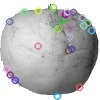
\includegraphics[width=0.1\textwidth]{ImageQ3a.jpeg} % 
  \end{figure}
  
  \vspace{12pt}

  \hrule 

  \vspace{12pt}
  The 100-dimensional vector obtained after performing K-means clustering on the keypoints dataset represents a compact encoding of the visual information contained in the training images. It is like summarizing each image with a list of 100 key characteristics that represent what makes each image unique. 
  
  \vspace{12pt}

  Example vector representing a fruit image from the training dataset: 
  [0 0 1 3 0 0 3 2 1 0 0 1 0 0 0 1 0 0 3 0 0 1 1 0 0 0 0 0 0 0 1 0 0 1 1 0 1 0 1 1 0 1 1 0 0 2 1 0 0 0 1 0 0 0 0 0 0 0 0 1 0 0 1 4 3 0 0 0 0 2 0 2 1 1 1 0 1 0 2 0 2 0 2 0 0 0 0 2 1 0 1 0 1 1 0 1 3 0 1 0]

  \vspace{12pt}

  Each element of the vector corresponds to the average position of all the data points assigned to that cluster, obtained from the K-means algorithm, capturing the most significant features shared among the keypoints across the entire dataset. By quantizing the keypoints into clusters, we reduce the dimensionality of the data while preserving the essential characteristics necessary for distinguishing between different images. 
   \vspace{12pt}

  In summary, this vector serves as a condensed representation of the image content, for efficient processing and analysis in subsequent stages of the SVM model.

  \vspace{12pt}

  \hrule 

  \vspace{12pt}

  Shape of training dataset D: (4665, 100)
  \vspace{12pt} 

  The shape of the training dataset is (4665, 100), indicating that it contains 4665 sample fruit images and each sample is represented by a 100-dimensional vector. This shape suggests that there are 4665 instances in the dataset, with each instance having 100 features. 

  \vspace{12pt}

  \hrule 

  \vspace{12pt}


\begin{figure}[H]
    \centering
    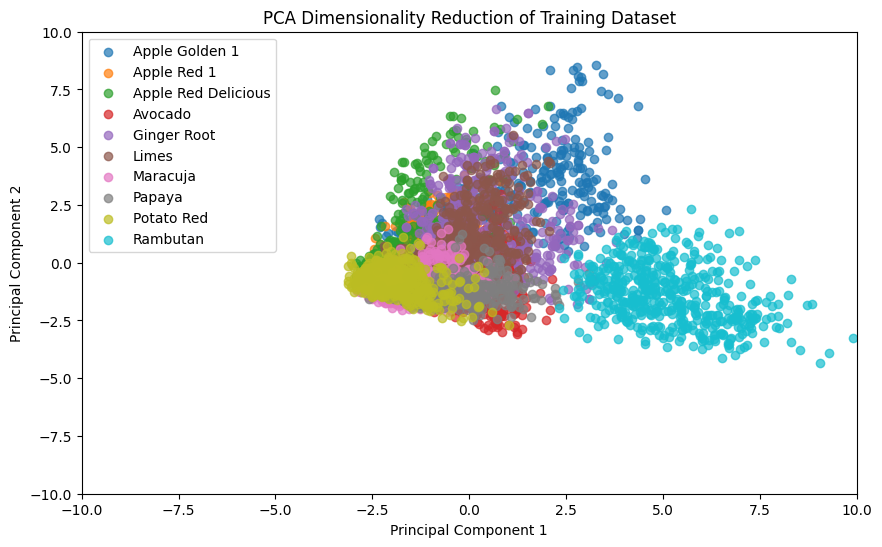
\includegraphics[width=0.7\textwidth]{Q3f.png} % 
  \end{figure}
  
  \vspace{12pt}

Plot of the 2D points using 10 different colors/symbols for data from the 10 classes: each point in the plot represents an instance from the dataset after performing Principal Component Analysis (PCA) dimensionality reduction. In other words, each point corresponds to a specific fruit image in the original dataset.
\vspace{12pt}

The PCA algorithm projects the original high-dimensional data onto a lower-dimensional space while preserving the maximum variance. Therefore, each point in the plot represents the same data instance as in the original dataset, but now represented in a two-dimensional space defined by the principal components.
\vspace{12pt}

The colors assigned to each point distinguishes the data from different fruit classes. This color mapping helps visualize how the different classes are distributed and separated in the reduced-dimensional space. Understanding the separation of classes helps to assess the effectiveness of the classification algorithm. If classes are well-separated in the reduced-dimensional space plot, it suggests that the data is easily separable, leading to better classification performance.

\vspace{12pt}

The clustering or overlapping of most classes indicates that they share similar feature representations in the reduced-dimensional space. This suggests that these classes may be closely related in terms of their features.
\vspace{12pt}

The Rambutan class (light blue) is positioned farther away from the clustered regions suggesting that it has distinct features compared to the other classes. This separation implies that the feature representations of Rambutan fruits are less similar to those of the other classes, leading to a more distinct cluster.

\vspace{12pt}

\hrule 

\vspace{12pt}

We perform the same steps on the testing dataset: 

\vspace{12pt}
  Example vector representing Image A for testing data: [0 5 0 0 0 0 0 0 2 1 0 0 0 0 0 1 0 1 0 0 3 0 0 0 0 4 0 0 0 0 0 2 1 1 2 2 1 0 1 3 1 0 0 2 0 0 0 0 0 2 1 4 0 2 0 2 0 0 0 1 6 1 0 2 1 0 0 0 0 0 0 2 10 0 1 0 1 2 0 0 0 0 1 1 1 0 0 0 0 1 0 0 0 0 1 0 0 0 0]
  \vspace{12pt}

      Shape of testing dataset D: (1542, 100)
      \vspace{12pt}

      \hrule 

      \vspace{12pt}

  
    
      Linear SVM Model Performance with Varying C Values: the SVM model was trained using different C parameter values to determine their impact on model performance. Here are the results obtained:

      \begin{table}[H]
        \centering
        \caption{Linear SVM Model Performance with Varying C Values}
        \begin{tabular}{@{}cccccc@{}}
            \toprule
            \textbf{C Value} & \textbf{Training Accuracy} & \textbf{Testing Accuracy} & \textbf{Train Error} & \textbf{Test Error} \\ 
            \midrule
             0.01 & 0.9353 & 0.6939 & 0.0647 & 0.3061 \\
              0.1 & 0.9674 & 0.6920 & 0.0326 & 0.3080 \\
              1.0 & 0.9871 & 0.6816 & 0.0129 & 0.3184 \\
             10 & 0.9961 & 0.6790 & 0.0039 & 0.3210 \\
             100 & 1.0000 & 0.6744 & 0.0000 & 0.3256 \\ 
            \bottomrule
        \end{tabular}
    \end{table}
      

    \vspace{12pt}

  
    \begin{figure}[H]
      \centering
      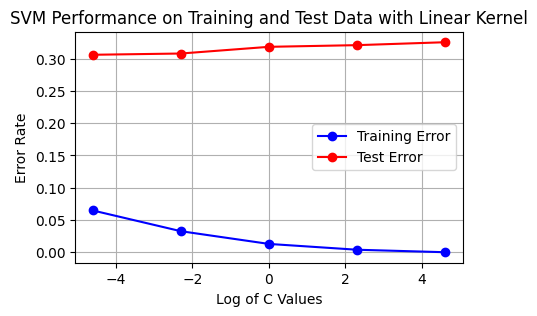
\includegraphics[width=0.5\textwidth]{graphQ5arr.png} % 
    \end{figure}
      
    \vspace{12pt}

    \begin{itemize}
      
    \item C Value: 0.01

    \item[] Training Accuracy: 0.9353
    \item[] Testing Accuracy: 0.6939
    \item[] With a very small value of C, the model demonstrates relatively high training and testing accuracies. However, the model might be underfitting, as indicated by the significant difference between training and testing accuracies.
    
    \item C Value: 0.1
    \item[]Training Accuracy: 0.9674
    \item[] Testing Accuracy: 0.6920
    \item[] As the C value increases, the training accuracy improves slightly. However, the testing accuracy starts to decline suggesting the potential for overfitting.
    
    \item C Value: 1.0
    \item[] Training Accuracy: 0.9871
    \item[] Testing Accuracy: 0.6816
    \item[] With a moderate C value, the training accuracy continues to improve, but the testing accuracy further declines. This indicates that the model is likely overfitting to the training data, as it fails to generalize well to unseen data.
    
    \item C Value: 10
    
    \item[] Training Accuracy: 0.9961
    \item[] Testing Accuracy: 0.6790
    \item[] At higher C values, the training accuracy reaches near-perfection. However, the testing accuracy decreases further, indicating significant overfitting and poor generalization.
    
    \item C Value: 100
    
    \item[] Training Accuracy: 1.0000
    \item[] Testing Accuracy: 0.6744
    \item[] With the highest C value, the model achieves perfect training accuracy but performs poorly on the testing data. This extreme overfitting highlights the limitations of the linear kernel in capturing the complexities of the dataset.
    
    \end{itemize}
    
    \vspace{12pt}
    In summary, the observed trend suggests that the linear kernel may not be the best fit for this dataset. The model struggles to find a balance between bias and variance, leading to poor generalization and overfitting as the C value increases. Alternative kernel functions or more complex models may be better suited to capture the underlying patterns in the data and improve performance.
   

  \vspace{12pt}
   \hrule 
  \vspace{12pt}


  \begin{figure}[H]
      \centering
      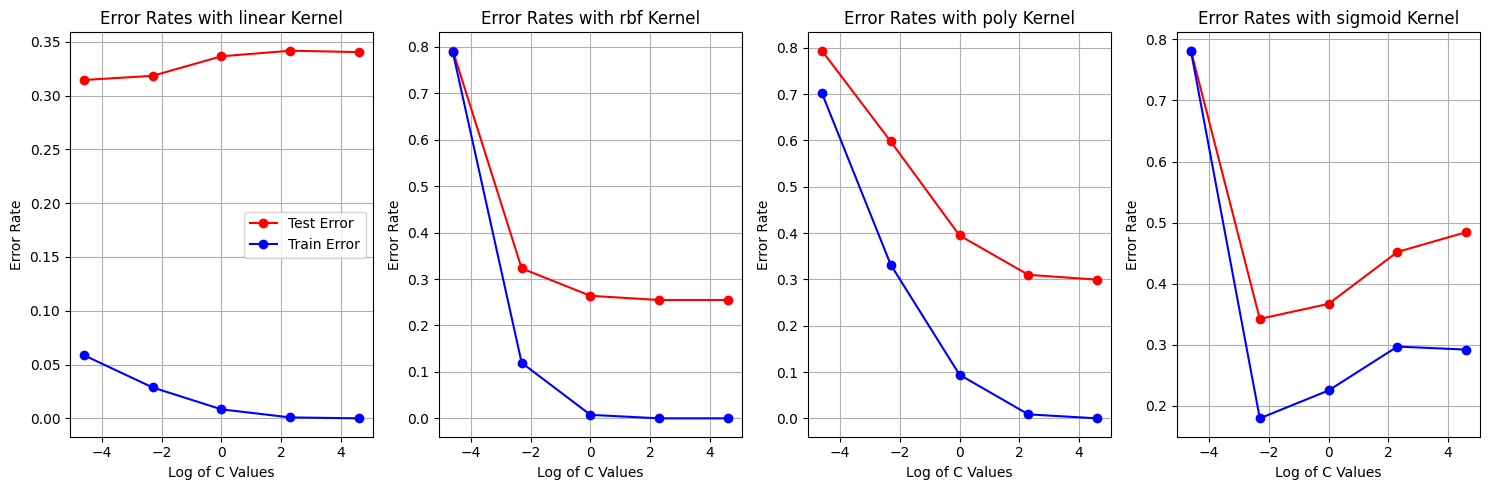
\includegraphics[width=1\textwidth]{graphQ5d1.png} % 
    \end{figure}
    
    \vspace{12pt}

    \begin{table}[H]
      \centering
      \caption{SVM Performance with Varying C Values}
      \label{tab:svm_performance}
      \begin{tabular}{@{}cccccc@{}}
                \toprule
         & C value & Training Accuracy & Testing Accuracy & Train Error & Test Error \\
        \midrule
        \multicolumn{6}{c}{\textbf{Kernel: linear}} \\
        \midrule
        & 0.01 & 0.941 & 0.685 & 0.059 & 0.315 \\
        & 0.1 & 0.971 & 0.682 & 0.029 & 0.318 \\
        & 1.0 & 0.992 & 0.663 & 0.008 & 0.337 \\
        & 10 & 0.999 & 0.658 & 0.001 & 0.342 \\
        & 100 & 1.000 & 0.660 & 0.000 & 0.340 \\
        \midrule
        \multicolumn{6}{c}{\textbf{Kernel: rbf}} \\
        \midrule
        & 0.01 & 0.212 & 0.208 & 0.788 & 0.792 \\
        & 0.1 & 0.880 & 0.677 & 0.120 & 0.323 \\
        & 1.0 & 0.992 & 0.736 & 0.008 & 0.264 \\
        & 10 & 1.000 & 0.745 & 0.000 & 0.255 \\
        & 100 & 1.000 & 0.745 & 0.000 & 0.255 \\
        \midrule
        \multicolumn{6}{c}{\textbf{Kernel: poly}} \\
        \midrule
        & 0.01 & 0.298 & 0.206 & 0.702 & 0.794 \\
        & 0.1 & 0.668 & 0.402 & 0.332 & 0.598 \\
        & 1.0 & 0.906 & 0.605 & 0.094 & 0.395 \\
        & 10 & 0.991 & 0.690 & 0.009 & 0.310 \\
        & 100 & 0.999 & 0.700 & 0.000 & 0.300 \\
        \midrule
        \multicolumn{6}{c}{\textbf{Kernel: sigmoid}} \\
        \midrule
        & 0.01 & 0.219 & 0.219 & 0.781 & 0.781 \\
        & 0.1 & 0.820 & 0.658 & 0.180 & 0.342 \\
        & 1.0 & 0.775 & 0.633 & 0.225 & 0.367 \\
        & 10 & 0.703 & 0.548 & 0.297 & 0.452 \\
        & 100 & 0.708 & 0.516 & 0.292 & 0.484 \\
        \bottomrule
      \end{tabular}
  \end{table}

  The best results for each kernel based on the least test error are: Linear kernel with C value of 0.01 (Test Error: 0.315), RBF kernel with C values of 10 and 100 (Test Error: 0.255), Poly kernel with C value of 100 (Test Error: 0.300), Sigmoid kernel with C value of 0.1 (Test Error: 0.342).

    
  \vspace{12pt}

  
  \hrule 
  \vspace{12pt}
    
  Plot of the best performance (lowest error rate) for each kernel. It identifies the best performing C value for each kernel based on the lowest error rate achieved.

  \begin{figure}[htbp]
    \centering
    \includegraphics[width=1\textwidth]{graphQ5er.png} % 
    
  \end{figure}


  \vspace{12pt}


  The graph illustrates the performance comparison of SVM using four different kernels: linear, rbf, poly, and sigmoid. The best error rate refers to the test error, which is the error rate calculated on the testing dataset. 
  
  \vspace{12pt}

  The results indicate that the RBF kernel with C=10 provides the best overall performance, achieving the highest testing accuracy of approximately 74.5\%. Additionally, it has the lowest test error rate 0.255 among all kernel-C combinations, indicating its effectiveness in generalizing to unseen data. The RBF kernel with C=10 also exhibits perfect training accuracy, suggesting a good balance between bias and variance, avoiding overfitting while capturing the underlying patterns in the data.


  \begin{figure}[H]
    \centering
    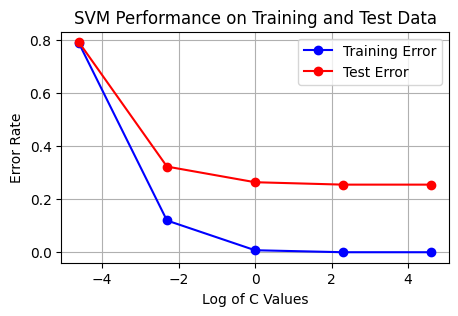
\includegraphics[width=0.5\textwidth]{graphQ5ar.png} % 
  \end{figure}
    
  \vspace{12pt}

  \begin{itemize}

    \item  C Value: 0.01:
    \item [] Testing accuracy: 0.2082
    \item [] This is the lowest testing accuracy observed in the table, indicating poor generalization performance of the SVM model.
    \item [] The model trained with this C value likely suffers from high bias, meaning it is underfitting the training data and failing to capture the underlying patterns in the data.
    \item C Value: 0.1:
    \item [] Testing accuracy: 0.6770
    \item [] There is a significant improvement in testing accuracy compared to the previous C value.
    \item [] While the model's performance has improved, it still exhibits some degree of underfitting, as indicated by the noticeable gap between training and testing accuracies.
    \item C Value: 1.0:
    \item [] Testing accuracy: 0.7361
    \item [] This represents a substantial increase in testing accuracy compared to the previous values of C.
    \item [] The model seems to have found a better balance between bias and variance, leading to improved generalization performance.
    \item C Value: 10 and 100:
    \item [] Testing accuracy: 0.7451 (identical for both C values)
    \item [] These two values of C yield the highest testing accuracy in the table.
    The model performs consistently well on unseen test data, suggesting that further increasing the complexity of the decision boundary (by reducing regularization) does not provide significant additional benefits.
  \end{itemize}
  
  \vspace{12pt}

  In the context of Support Vector Machines (SVM), C values represent the regularization parameter. Regularization is a technique used to prevent overfitting by adding a penalty term to the loss function. In SVM, the parameter C controls the trade-off between maximizing the margin (decision boundary) and minimizing the classification error. A small C value allows for a larger margin but may misclassify some points (soft margin). A large C value penalizes misclassifications heavily, potentially resulting in a smaller margin (hard margin). In essence, C values determine the balance between achieving a low training error and generalizing well to unseen data.

  \vspace{12pt}


    In summary, the testing accuracies demonstrate the impact of the regularization parameter C on the SVM model's ability to generalize to unseen data. Lower values of C may lead to underfitting and poor performance, while higher values can improve performance up to a certain point before potentially overfitting the model to the training data. The optimal choice of C depends on balancing bias and variance to achieve the best generalization performance.

  \vspace{12pt}
  


  \begin{table}[H]
    \centering
    \caption*{Table with Predicted Class (kernel: RBF, C=10)}
    \label{tab:images}
    \begin{tabular}{|c|c|c|c|c|}
        \hline
        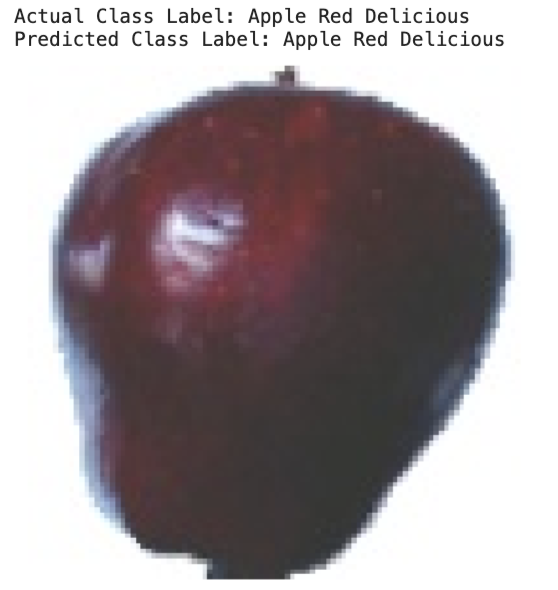
\includegraphics[width=0.17\textwidth]{image1.png} &
        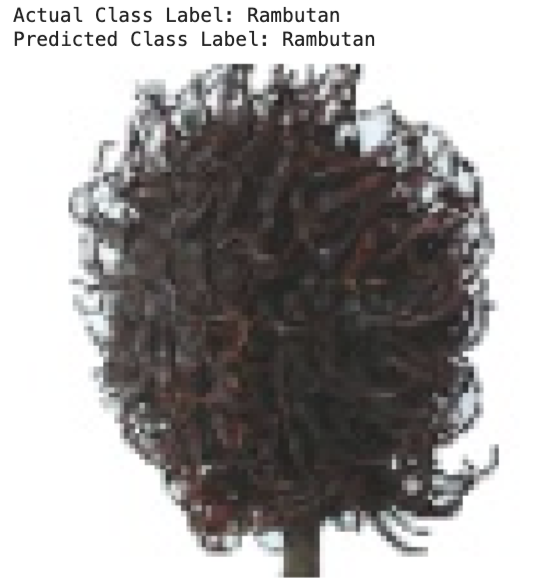
\includegraphics[width=0.17\textwidth]{image2.png} &
        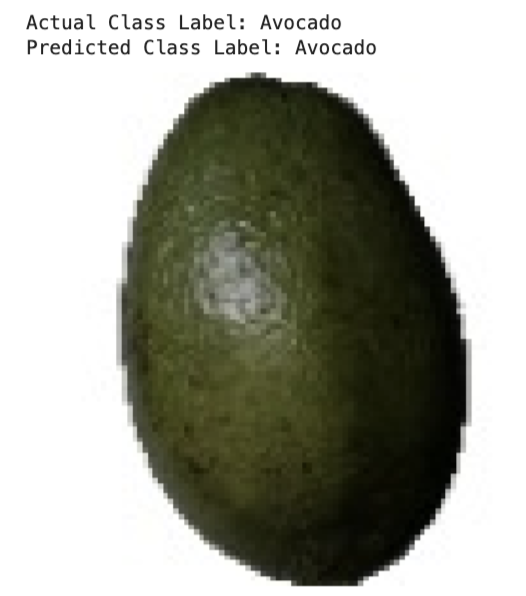
\includegraphics[width=0.17\textwidth]{image4.png} &
        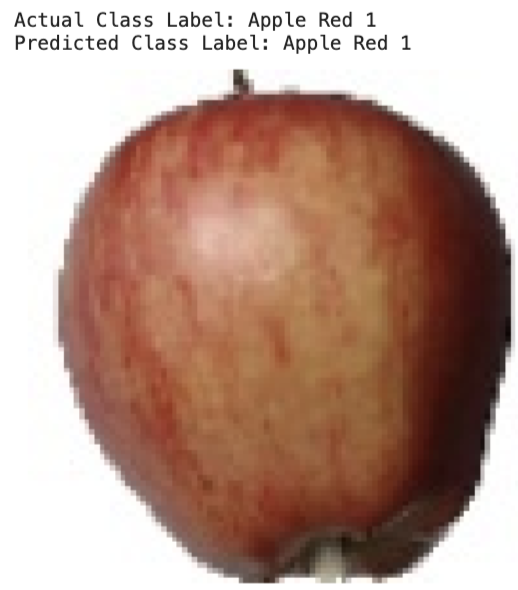
\includegraphics[width=0.17\textwidth]{image5.png} &
        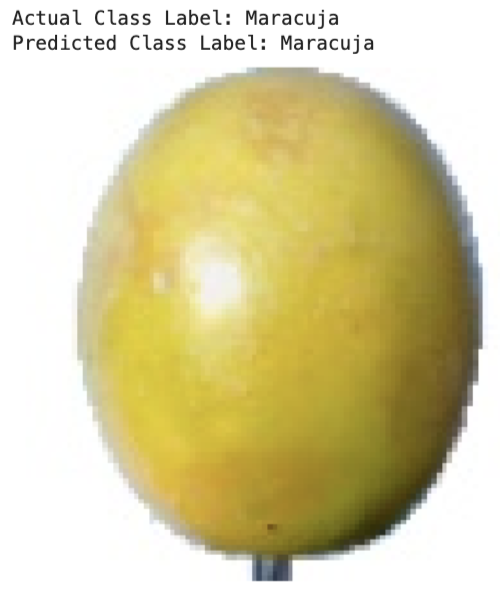
\includegraphics[width=0.17\textwidth]{image3.png} \\
        \hline
        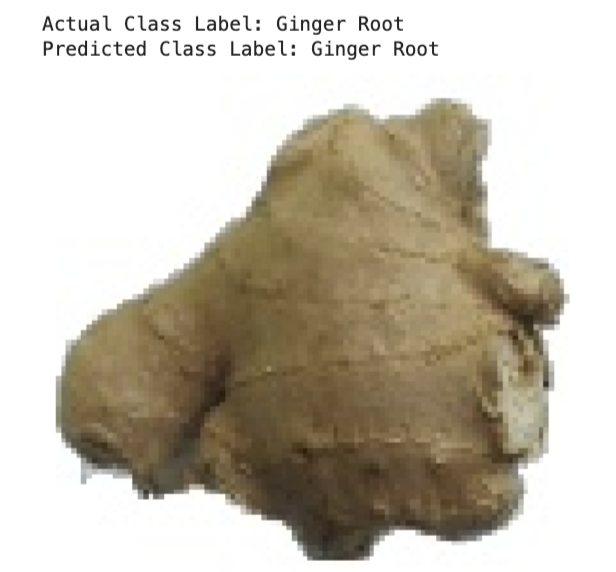
\includegraphics[width=0.17\textwidth]{image7.png} &
        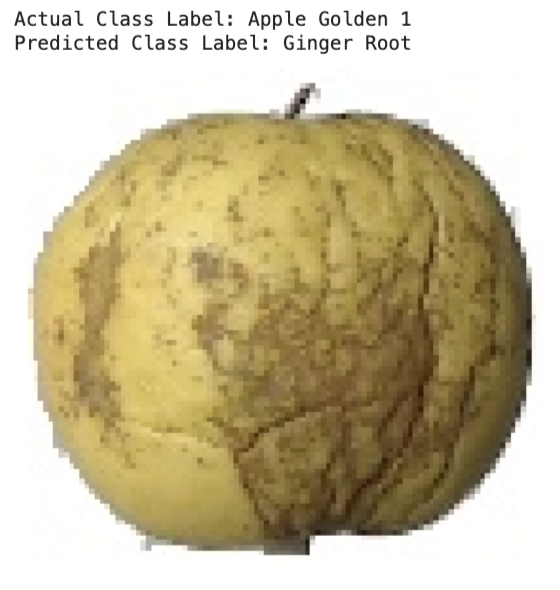
\includegraphics[width=0.17\textwidth]{image6.png} &
        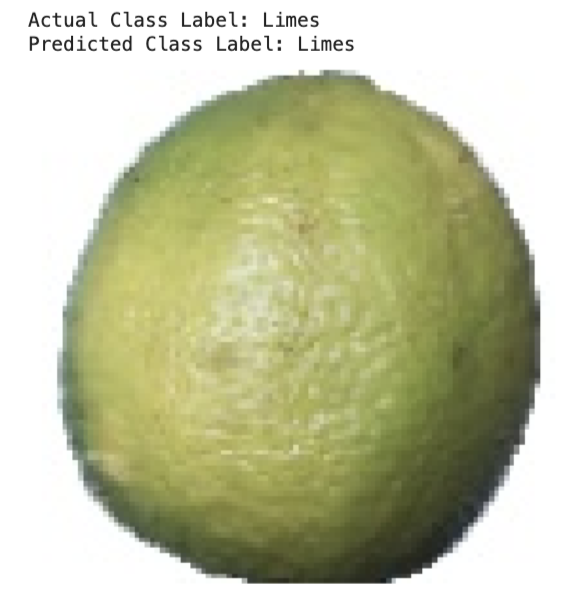
\includegraphics[width=0.17\textwidth]{image8.png} &
        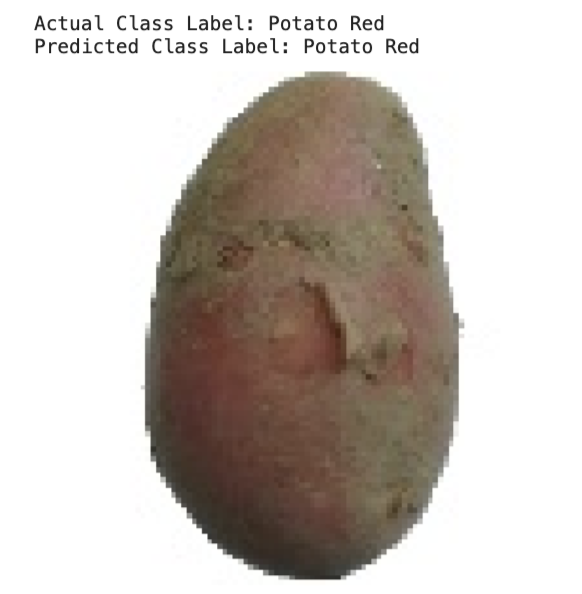
\includegraphics[width=0.17\textwidth]{image9.png} &
        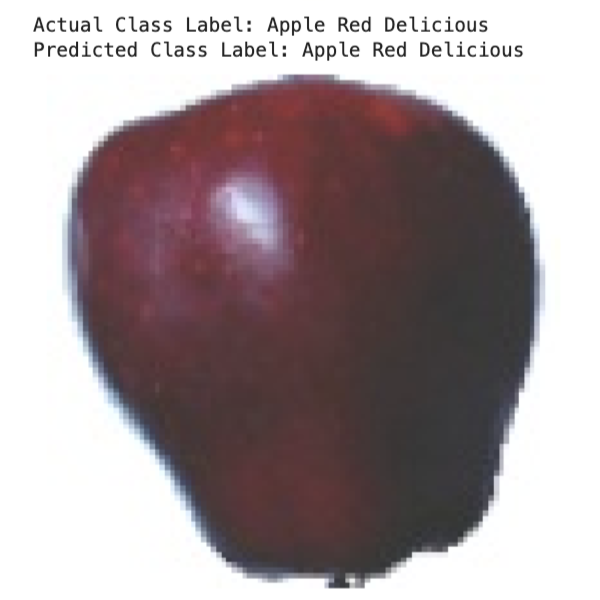
\includegraphics[width=0.17\textwidth]{image10.png} \\
        \hline
    \end{tabular}
\end{table}

In the table above, the predicted classes for a selection of six fruit images align with their actual classes, with one exception. Among these images, there was a discrepancy: an image labeled as Apple Golden 1 was instead predicted to be Ginger Root. 

\vspace{12pt}

\vspace{12pt}

  {\Large \textbf {Questions 6 to 8}}
  \vspace{12pt}


  The validation loss decreases consistently with each epoch (graph 6(a)), indicating that the model is learning effectively from the training data. Simultaneously, the training accuracy increases steadily, reaching 100\% accuracy by the 4th epoch. This suggests that the model is fitting the training data very well, achieving perfect accuracy.

  \vspace{12pt}

  \begin{table}[H]
    \centering
    \caption{Performance Metrics for Simple Convolutional Neural Network}
    \label{tab:cnn_performance}
    \begin{tabular}{@{}cccccc@{}}
      \toprule
      \textbf{Epoch} & \textbf{Training Loss} & \textbf{Training Accuracy} & \textbf{Validation Loss} & \textbf{Validation Accuracy} \\
      \midrule
      1 & 0.6253 & 0.7912 & 0.1014 & 0.9418 \\
      2 & 0.0557 & 0.9850 & 0.0454 & 0.9741 \\
      3 & 0.0071 & 0.9998 & 0.0182 & 1.0000 \\
      4 & 0.0024 & 1.0000 & 0.0120 & 1.0000 \\
      5 & 0.0013 & 1.0000 & 0.0060 & 1.0000 \\
      6 & 0.0009 & 1.0000 & 0.0059 & 1.0000 \\
      7 & 0.0006 & 1.0000 & 0.0054 & 1.0000 \\
      8 & 0.0005 & 1.0000 & 0.0034 & 1.0000 \\
      9 & 0.0003 & 1.0000 & 0.0031 & 1.0000 \\
      10 & 0.0003 & 1.0000 & 0.0033 & 1.0000 \\
      11 & 0.0002 & 1.0000 & 0.0030 & 1.0000 \\
      12 & 0.0002 & 1.0000 & 0.0027 & 1.0000 \\
      13 & 0.0002 & 1.0000 & 0.0026 & 1.0000 \\
      14 & 0.0001 & 1.0000 & 0.0027 & 1.0000 \\
      15 & 0.0001 & 1.0000 & 0.0024 & 1.0000 \\
      16 & 0.0001 & 1.0000 & 0.0019 & 1.0000 \\
      17 & 0.0001 & 1.0000 & 0.0013 & 1.0000 \\
      18 & 0.0001 & 1.0000 & 0.0015 & 1.0000 \\
      19 & 0.0001 & 1.0000 & 0.0016 & 1.0000 \\
      20 & 0.0001 & 1.0000 & 0.0015 & 1.0000 \\
      \bottomrule
  \end{tabular}
\end{table}


  The validation accuracy, evaluated on the test data, improves significantly with each epoch. It reaches 100\% (graph 6(a))accuracy by the 3rd epoch and maintains this perfect accuracy throughout the remaining epochs. This indicates that the model generalizes well to unseen data, achieving optimal performance on both the training and test datasets.

  \vspace{12pt}



  \begin{figure}[H]
    \centering
    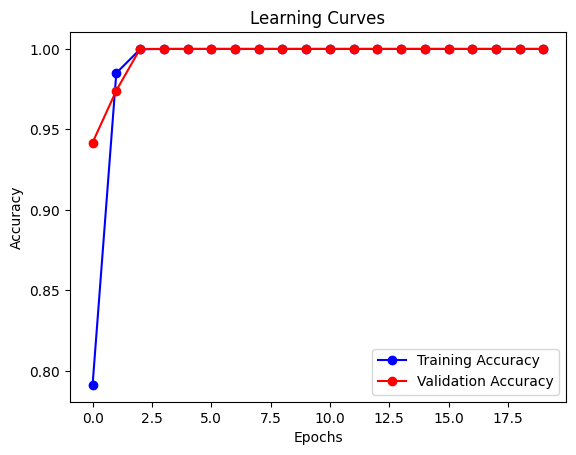
\includegraphics[width=0.5\textwidth]{graphQ6r.png} % 
    \caption{6(a)}
  \end{figure}

  \vspace{12pt}

  Given the perfect accuracy achieved, the learning curves appear as two flat lines at the top of the graph after a few epochs (graph 6(a)). Overall, the CNN model demonstrates excellent learning capabilities, effectively capturing patterns in the data and achieving perfect classification accuracy on both training and test datasets.

  \vspace{12pt}

  \hrule

  \vspace{12pt}

  Throughout the 10 epochs of training, the training loss consistently decreases (graph 7(b)), indicating effective learning from the training data. The training accuracy quickly reaches 100\%, demonstrating that the model is successfully fitting the training data.

  \vspace{12pt}

  \begin{table}[H]
    \centering
    \caption{Performance Metrics for Transfer Learning with ResNet18}
    \label{tab:resnet18_performance}
    \begin{tabular}{@{}cccc@{}}
      \toprule
      \textbf{Epoch} & \textbf{Training Loss} & \textbf{Training Accuracy} & \textbf{Validation Accuracy} \\
      \midrule
      1 & 0.387 & 0.945 & 1.000 \\
      2 & 0.042 & 1.000 & 1.000 \\
      3 & 0.020 & 1.000 & 1.000 \\
      4 & 0.013 & 1.000 & 1.000 \\
      5 & 0.009 & 1.000 & 1.000 \\
      6 & 0.007 & 1.000 & 1.000 \\
      7 & 0.005 & 1.000 & 1.000 \\
      8 & 0.004 & 1.000 & 1.000 \\
      9 & 0.004 & 1.000 & 1.000 \\
      10 & 0.003 & 1.000 & 1.000 \\
      \bottomrule
  \end{tabular}

  \end{table}

  The validation accuracy, evaluated on the test set, remains consistently at 100\% throughout the training process (graph 7(b)). This indicates that the model generalizes well to unseen data and maintains high accuracy on the test set, suggesting robust performance.

  \begin{figure}[H]
    \centering
    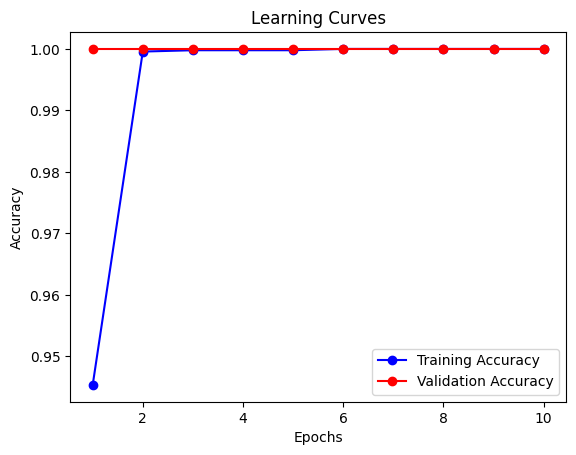
\includegraphics[width=0.5\textwidth]{graphQ7r.png} % 
    \caption{7(b)}
  \end{figure}

  \vspace{12pt}

  The validation accuracy curve shows as a flat line at the top of the graph, representing perfect validation accuracy. This demonstrates that the model achieves optimal performance without overfitting, as both training and validation accuracies converge to 100\% (graph 7(b)). 

  \vspace{12pt}

  \hrule

  SVM Training Accuracy: 1.0

  SVM Test Accuracy: 1.0
  \hrule 

  \vspace{12pt}

  The SVM prediction model trained, on the hyperparameters that resulted in best results (C=10, kernel: RBF), and using features extracted from the ResNet18 model, achieves perfect accuracy on both the training and test sets, with training accuracy and test accuracy both reaching 100\%. 

  \vspace{12pt}
  
  The SVM model achieves 100\% accuracy on the training set, indicating that it perfectly separates the classes based on the extracted features. This suggests that the SVM effectively learns the decision boundary to classify the training data without any errors. Similarly, the SVM model achieves 100\% accuracy on the test set, implying that it generalizes well to unseen data. This indicates that the model's performance is not limited to the training data and can accurately classify new instances based on the learned decision boundary.

  \vspace{12pt}

  Overall, the perfect training and test accuracies suggest that the SVM model, trained using features extracted from the ResNet18 model, effectively captures the discriminative information present in the data. This indicates the robustness and effectiveness of the feature extraction process and the SVM classifier in accurately classifying the 10 fruit classes.


  \vspace{12pt}

  \hrule

  \vspace{12pt}

  The results of fine-tuning the pre-trained ResNet18 model show fluctuations over epochs. It starts high, reaches perfect accuracy (1.0) in the third epoch, but drops towards the second and fourth epochs. This behavior suggests that the model may be overfitting the training data, especially evident in the drop and fluctuations of validation accuracy. \textit{"Low error rates and a high variance are good indicators of overfitting"} \cite{ibm_overfitting}.


\begin{table}[H]
  \centering
  \caption{Performance Metrics for Transfer Learning via Fine-Tuning with ResNet18}
  \label{tab:resnet18_finetuning_performance}
  \begin{tabular}{@{}cccc@{}}
    \toprule
    \textbf{Epoch} & \textbf{Training Loss} & \textbf{Training Accuracy} & \textbf{Validation Accuracy} \\
    \midrule
    1 & 0.304 & 0.901 & 0.989 \\
    2 & 0.143 & 0.956 & 0.749 \\
    3 & 0.095 & 0.969 & 1.000 \\
    4 & 0.050 & 0.984 & 0.747 \\
    5 & 0.023 & 0.994 & 0.987 \\
    6 & 0.017 & 0.995 & 0.520 \\
    7 & 0.102 & 0.976 & 0.786 \\
    8 & 0.113 & 0.960 & 0.591 \\
    9 & 0.033 & 0.990 & 0.756 \\
    10 & 0.013 & 0.998 & 1.000 \\
    \bottomrule
\end{tabular}
\end{table}

  \vspace{12pt}

  While the model achieves high validation accuracy in epoch 10/10, the fluctuations in validation accuracy indicate instability in model performance. 

  \begin{figure}[H]
    \centering
    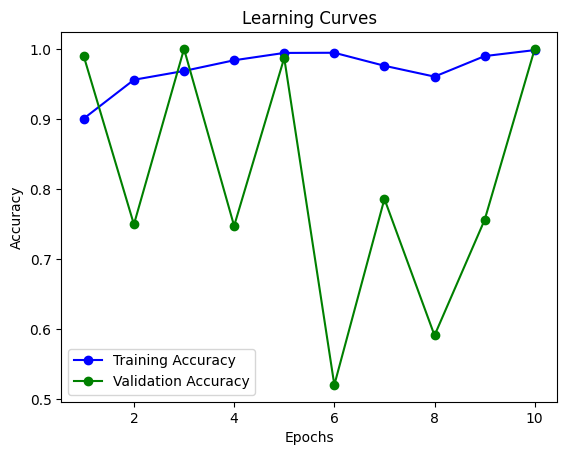
\includegraphics[width=0.5\textwidth]{graphQ8r.png} % 
    \caption{8(b)}
  \end{figure}


{\Large \textbf {Question 9}}
\begin{itemize}[]
  \item[(a)] \textit{"If the training data has a low error rate and the test data has a high error rate, it signals overfitting"} \cite{ibm_overfitting}.
  \item[]  Overall, the results suggest that the three models have successfully learned the underlying patterns in the data and generalize well to new samples.
  \item[] The CNN model achieves high training and validation accuracies throughout the training epochs. 
  \item[] Similar to the CNN model, the ResNet18 model also achieves high training and validation accuracies. Overfitting is not evident as the validation accuracy remains consistently high across epochs. Therefore, the test accuracy before overfitting occurs would correspond to the validation accuracy at the last epoch, which is 1.000. 
  \item[] Overfitting is indicated when the validation accuracy starts to deviate from the training accuracy or decreases. In this case, with the Transfer Learning via Fine-Tuning with ResNet18 model we observe a slight fluctuation in validation accuracy starting from epoch 2/10, suggesting potential overfitting. Therefore, the test accuracy before overfitting occurs would correspond to the validation accuracy at epoch 1/10, which is 0.989
  \item[] 
  \item[(b)] Comparing the best results for each model, we can see that CNN and transfer learning models achieved the highest test accuracies of 1.000, indicating perfect classification on the test dataset. Therefore, these approaches tie for the best performance in terms of test accuracy and low error rate.
  \item[] 
  \begin{table}[H]
    \centering
    \caption{Comparison of Test Accuracy for Different Approaches}
    \label{tab:results}
    \begin{tabular}{@{}lll@{}}
    \toprule
    \textbf{Approach} & \textbf{Test Accuracy}  \\ \midrule
    Deep Learning - CNN (epoch 20/20) & 1.000  \\
    Transfer Learning - Feature Extraction (epoch 10/10) & 1.000  \\
    Transfer Learning - Fine-Tuning (epoch 10/10) & 1.000  \\ \bottomrule
    \end{tabular}
    \end{table}

    \item[] We could instead consider the epochs before overfitting occurs for each model to provide a fair comparison of their test accuracies.
    \begin{table}[H]
      \centering
      \caption{Comparison of Test Accuracy Before Overfitting for Different Approaches}
      \label{tab:results}
      \begin{tabular}{@{}lll@{}}
      \toprule
      \textbf{Approach} & \textbf{Test Accuracy}  \\ \midrule
      Deep Learning - CNN (epoch 20/20) & 1.000  \\
      Transfer Learning - Feature Extraction (epoch 10/10) & 1.000  \\
      Transfer Learning - Fine-Tuning (epoch 1/10) & 0.989  \\ \bottomrule
      \end{tabular}
      \end{table}
      \item[] Here the best performing model is the CNN and Transfer Learning - Feature Extraction models with an accuracy of 1.00

  \item[(c)] The performance result that surprises me the most is the test accuracy of 1.000 (or 100\%) achieved. This level of accuracy indicates that the models achieved perfect classification on the test data, which is quite remarkable.
  \item [] The reason for my surprise is that achieving perfect accuracy, especially across all test samples, is rare in real-world scenarios. It suggests that the models have effectively learned the underlying patterns in the data and generalized well to unseen examples. However, such high accuracy rates may also indicate overfitting, where the models have memorized the training data too well, leading to poor performance on new data. This is mainly a cause of concern because the testing dataset is very similar to the training dataset in the case of the fruit images available with this project.
  
  \item[] Therefore, while the perfect accuracy is impressive, it also prompts further investigation into the robustness and generalization capabilities of the models to ensure they perform well in diverse real-world scenarios.  




\end{itemize}

\bibliographystyle{plain} % Choose a bibliography style
\bibliography{biblio.bib} % Name of your .bib file without extension

\end{document}